\chapter{Background}
\label{chap:background}

In this chapter the needed background for this work will be shown.
Therefore, first the AutoML concept in general will be explained.
Then the optimization techniques that are used in AutoML systems will be shown.
These optimization techniques require metrics as input.
So, the metrics that are available for clustering will be presented.
Afterwards the concept of Meta-learning will be described.

\section{AutoML}
The problem of \gls{AutoML} is to produce automatically, so without human input, test set predictions for a given test set within a resource budget $b$.
This can be formally defined as shown in \Cref{def:automl}.

\begin{definition}[\gls{AutoML} problem]
\label{def:automl}
For $i = 1, \dots, n+m$ let $x_i \in \mathbb{R}^d$ denote a feature vector and $y_i \in Y $ the corresponding target value.
Given training data $D_{train} = \lbrace (x_1, y_1), \dots, (x_n, y_n) \rbrace $ and the feature vectors $x_{n+1, \dots, n+m}$ of a test dataset $D_{test} = \lbrace (x_{n+1}, y_{n+1}), \dots, (x_{n+m}, y_{n+m})  \rbrace$ drawn from same underlying distribution, as well as a ressource budget $b$ and a loss metric $\mathbb{L}(\cdot, \cdot)$, the \gls{AutoML} problem is to automatically produce test set predictions $\hat{y}_{n+1}, \dots, \hat{y}_{n+m}$ such that the loss 
\begin{equation*}
    \frac{1}{m} \sum_{j=1}^m \Lcurv(\hat{y}_j, y_j)
\end{equation*}
is minimized.
\end{definition}


Many \gls{AutoML} systems do not directly address the problem described in \Cref{def:automl}, but they see the \gls{AutoML} problem as \gls{CASH} problem \cite{Feurer2015EfficientLearning,  Kotthoff2017Auto-WEKAWEKA}. 
This is because the main problems of \gls{AutoML} are that first there is no single algorithm that performs best on every dataset and the choice of hyperparameter is crucial for the performance of an algorithm.
The \gls{CASH} problem is formally defined in \Cref{def:cash}.

\begin{definition} [\gls{CASH} problem]
\label{def:cash}
Let $A^(1), \dots, A^(R)$ be a set of algorithms, where the hyperparameters of each algorithm have the domain $\Lambda^(i)$.
Alos, let $ D_{train} =  \lbrace (x_1, y_1), \dots, (x_n, y_n) \rbrace$ be a training set which is split into k  disjunct cross-validation folds $\lbrace D^{(1)}_{valid}, \dots, D^{(k)}_{valid} \rbrace$ and $\lbrace D^{(1)}_{train}, \cdots, D^{(k)}_{train} \rbrace$  such that $D^{(i)}_{train} = D_{train} \textbackslash D^{(i)}_{valid}$ for $i=1, \dots, k$.
Finally, let $L( A^{(i)}_{\lambda}, D^{(i)}_{train}, D^{(i)}_{valid})$ denote the loss that algorithm $A^{(i)}$ has on $D^{(i)}_{valid}$ when trained on $D^{(j)_{train}}$ with hyperparameters $\lambda$.
Then, the \gls{CASH} problem is to find the joint algorithm and hyperparameter setting that minimizes the loss:
\begin{equation*}
    A^*, \lambda^* \in \underset{A^{(j)}\in A, \lambda \in \Lambda^{(j)}}{argmin} \frac{1}{k} \sum_{i=1}^k \Lcurv(A^{(j)}_{\lambda}, D^{(i)}_{train}, D^{(i)}_{valid})
\end{equation*}

\end{definition}



\section{Hyperparameter Optimization Techniques for Classification}

\begin{itemize}
    \item Hyperparameter optimization in general, describe the problem of finding parameter configuration that maximizes the validation performance.
    \item 
\end{itemize}
In this section methods for the optimization of hyperparameters that are used in AutoML systems will be described.

Most of the methods have three steps in common, which are:
\begin{enumerate}
    \item Run the current model.
    \item Evaluate the results of the current model according to a metric.
    \item Select the next model that should be run.
\end{enumerate}
The difference in the methods is how they select the next model that will be run, so step 3 above. 

The methods that will be presented are shown in \cref{fig:hpo} and can generally be divided into three categories \cite{Li2017Hyperband:Optimization,BergstraAlgorithmsOptimization, Falkner2018BOHB:Scale, Feurer2015EfficientLearning}:
\begin{figure}
    \centering
    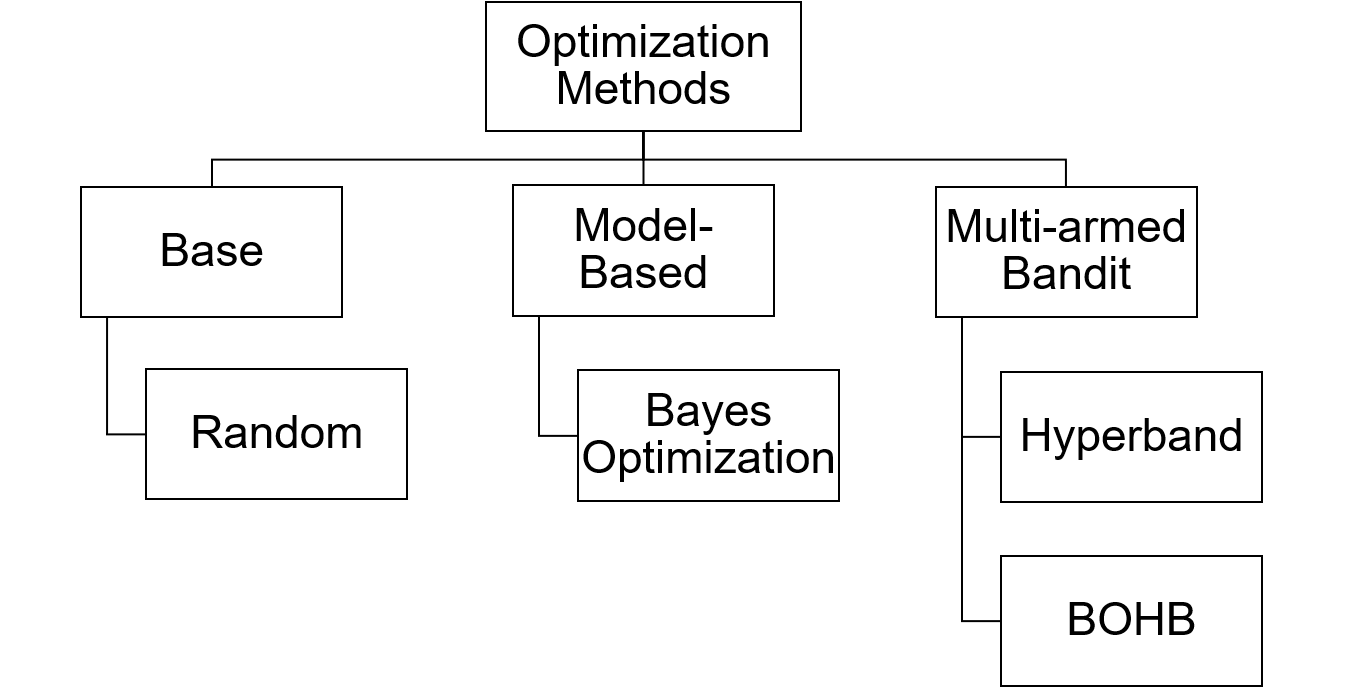
\includegraphics[width=0.5\textwidth]{data/HPO_methods.png}
    \caption{Overview of the hyperparameter optimization methods that will be described.}
    \label{fig:hpo}
\end{figure}
\begin{itemize}
    \item \textbf{Base}: Methods that are basically used like Random-search.
    Like the name suggests, Random-search is running random configurations and evaluates them.
    \item \textbf{Sequential model-based}: Methods that create a model of the hyperparameters to predict the best hyperparameters.
    One representative of this class is the \gls{BHO}
    \item \textbf{Multi-armed Bandit}: These methods try to sample a lot of configurations in parallel with a very low budget for each configuration.
    Examples for this class are Hyperband and \gls{BOHB}, which is a combination of \gls{BHO} and Hyperband.
\end{itemize}

In the following these methods will be described in more detail.
Of course, there are also other methods like gradient-based methods, but in the following only those methods will be presented that have proven to work well in the AutoML systems.


\subsection{Random}

\begin{itemize}
    \item One of the most simple Hyperparameter optimization methods is Random \cite{Bergstra:2012:RSH:2503308.2188395}.
    \item Though can be very effective, especially if the search space is not very large.
    \item Performs in general better than Gridsearch.
    \item Fails for large and high-dimensional parameter spaces.
    
\end{itemize}

\subsection{Bayes Optimization}

\begin{itemize}
    \item Model-based method that relies on a statistical model and an acquisition function \cite{ShahriariTakingOptimization, Frazier2018AOptimization, SnoekPracticalAlgorithms}.
    Goal of acquisition function is to find a sample that should be evaluated next.
    Should make trade-off between exploration and exploitation.
    \item Only a framework, several implementations with different models and acquisition functions.
    \item Surrogate model about how the objective function (parameter configuration to metric value).
    \item An example for an often used statistical model are Gaussian Processes (GP) \cite{ShahriariTakingOptimization}.
    \item Goal is to approximate this model by samples.
    \item The steps are:
    \begin{itemize}
        \item select next parameter configuration that maximizes the acquisition function.
        \item Run model with these parameter configuration.
        \item Evaluate the configuration, so calculate metric(configuration).
        \item Update the model.
    \end{itemize}
    \item An example for this procedure is shown in \cref{fig:BOExample}. 
    
    \begin{figure}
        \centering
        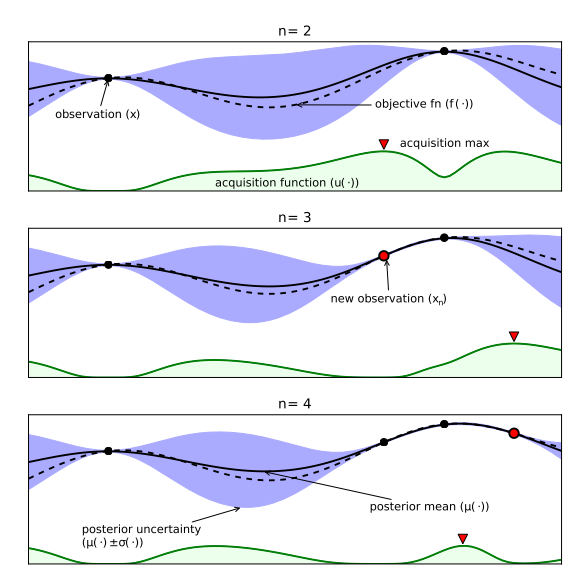
\includegraphics{graphics/bayes_optimization_example.png}
        \caption{Example of the Bayesian Optimization procedure \cite{ShahriariTakingOptimization}.}
        \label{fig:BOExample}
    \end{figure}
    \item Example for an acquisition function is the \gls{EI}:
    \begin{equation}
        a(x) = \int max(0, \alpha -f(x)) dp(f|D)
    \end{equation}
    Here $\alpha$ is the currently best observed value.
    \item One implementation of the Bayes optimization is the Tree Parzen Estimator (TPE) \cite{BergstraAlgorithmsOptimization}, which uses a density kernel estimator.
    
    \item Should only be used if f has no closed form or is expensive to evaluate.
    \item Sequential, so no parallelization.
    \item Only good after some samples, for less samples random could be better.
\end{itemize}

\subsection{Hyperband}

Hyperband \cite{Li2017Hyperband:Optimization} is a multi-armed bandit method that relies on \gls{SH} \cite{Jamieson2015Non-stochasticOptimization}.
The general algorithm is shown in \cref{fig:HBAlgorithm}.
\begin{figure}
    \centering
    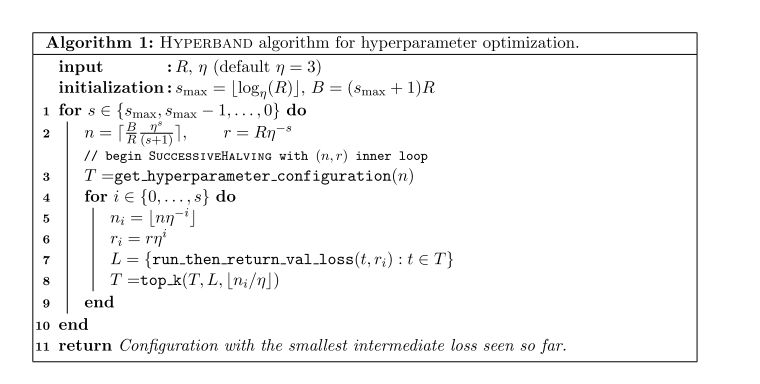
\includegraphics[width=\textwidth]{graphics/hyperband_algorithm.png}
    \caption{Overview of the Hyperband algorithm \cite{Li2017Hyperband:Optimization}.}
    \label{fig:HBAlgorithm}
\end{figure}

\begin{itemize}
    \item Gets as input the maximum budget for one configuration and $\eta$, which controls the amount of configurations that are discarded after each round of \gls{SH}.
    \item The general idea is to run many \gls{SH} runs.
    \item One SH run consists of many iterations. First random configurations are sampled.
    The number of configurations should be chosen in such a way that the minimum budget can be distributed equally over all configurations.
\end{itemize}

\subsection{Bayesian Optimization and Hyperband}

\gls{BOHB} is a combination of the Bayesian Optimization and the Hyperband method.
Instead of random sampling of configurations in the different \gls{SH} iterations of Hyperband, \gls{BOHB} uses Bayesian Optimization to fit a model and to select the configurations.
 

\section{Clustering Algorithms}

\begin{itemize}
    \item What is clustering
    \item what is partitional clustering
    \item which partitional clustering algorithms exist
    \item shortly explain the algorithms that are used in the implementation (GMM, KMeans, KMedoids)
\end{itemize}

\section{Clustering Metrics}
\begin{itemize}

    \item Metric Types: internal, external, relative (?)
    \item explain how they work and use show metrics that are used in the concept/implementation.
\end{itemize}

\section{Meta-learning}

Meta-learning \cite{Brazdil2010MetalearningMining.} is the task of learning to learn.
In the area of machine learning it can be used to learn algorithms and their configurations from previous tasks.
For this, it typically includes an offline and an online phase.
The basic workflow is shown in \cref{fig:metalearningArch}.
\begin{figure}
    \centering
    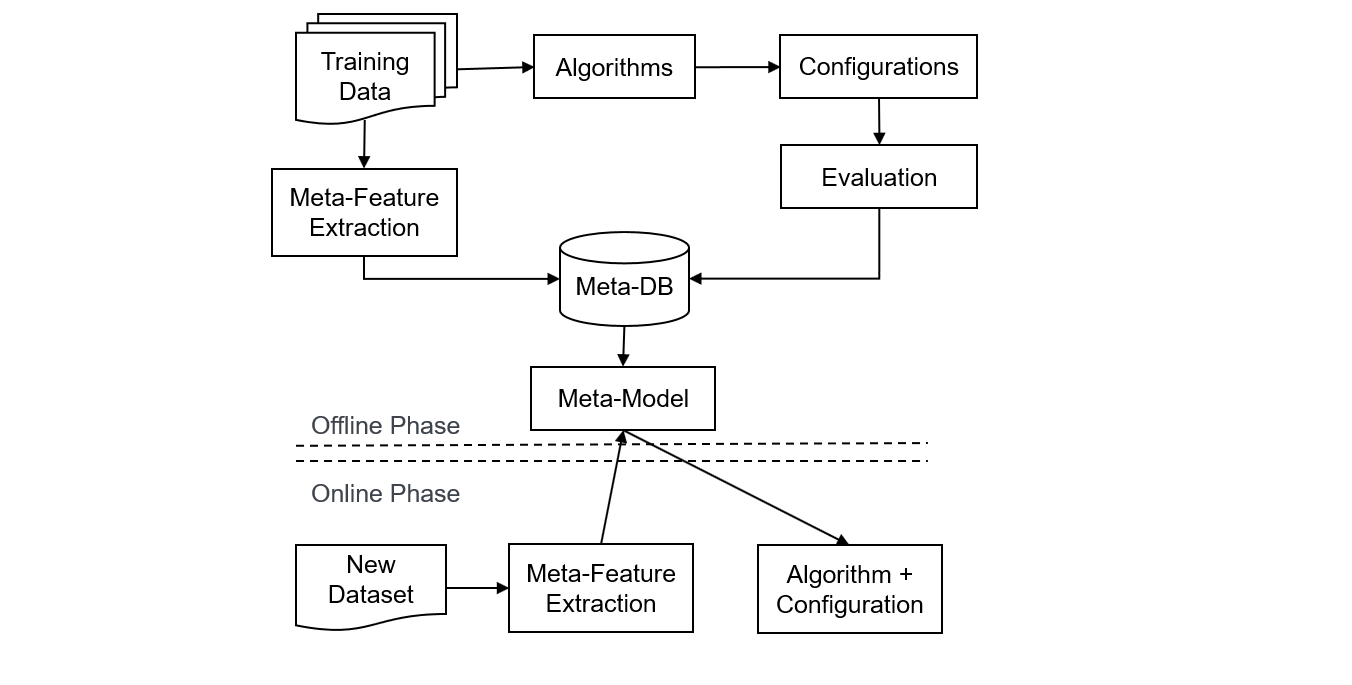
\includegraphics[width=\textwidth]{graphics/metalearning_general_architecture.png}
    \caption{General architecture of meta-learning, divided into offline and online phase.}
    \label{fig:metalearningArch}
\end{figure}

\begin{itemize}
    \item In an offline phase, training data is needed (which represents previous tasks).
    \item From this training data, \textit{meta-features} are extracted.
    Describe characteristics of the dataset.
    Example can be number of instances or number of attributes.
    \item meta-features of a dataset are saved in a database (meta-db in the figure).
    \item Then for the dataset, different algorithms with different configurations are run and evaluated.
    The configurations as well as the result of the evaluations are also stored in the meta-db.
    From meta-db information meta-learner can be derived.
    \item Online Phase: If new dataset, then first have to extract meta-features.
    \item Meta-features are input for meta-learner.
    \item Meta-learner suggests promising algorithm with configuration based on the meta-db knowledge.
    \item One possibility is to find the most similar dataset according to meta-features and then take best known algorithm and configuration from meta-db.
    \item This would correspond to a k-Nearest-Neighbor classifier with $k=1$.
    \item Question is which meta-features should be used.
    \item Meta-features can be categorized into five groups \cite{Rivolli2018TowardsMeta-learning}:
    \begin{itemize}
        \item \textbf{Simple}: Can be directly extracted from the data and include measure like the number of instances or the number of attributes.
        \item \textbf{Statistical}: Measure statistical information about the data.
        They include measure like mean, median, standard deviation etc.
        \item \textbf{Information-theoretic}: Based on entropy and capture the information and the complexity in the data.
        An example is the attribute entropy.
        \item \textbf{Model-based}: This group of meta-features use structural properties of machine learning models.
        For example they build a decision tree from the data and the number of leaves of that tree is one meta-feature.
        \item \textbf{Landmarking}: The landmarking meta-features use the performance of simple classifiers like Naive Bayes as meta-features.
    \end{itemize}
    
    \item Landmarking and model-based cannot be used for clustering since we are assuming in the online phase of meta-learning that there are no class labels. 
    \item Other groups also contain meta-features with class labels, e.g., the number of classes. For this work only those without class labels are interesting.
\end{itemize}